\documentclass[12pt]{article} % use larger type; default would be 10pt
\usepackage[czech]{babel}
\usepackage[utf8]{inputenc} % set input encoding (not needed with XeLaTeX)

%%% PAGE DIMENSIONS
\usepackage{geometry} % to change the page dimensions
% \usepackage[left=2cm,right=2cm,top=2cm,bottom=2cm]{geometry}
\geometry{a4paper}
% \geometry{margin=2in} % for example, change the margins to 2 inches all round
% \geometry{landscape} % set up the page for landscape

\usepackage{graphicx} % support the \includegraphics command and options
\usepackage{wrapfig} % support the wrapfigure section

\usepackage{hyperref} % links in \tableofcontents
\hypersetup{
	colorlinks,
	citecolor=black,
	filecolor=black,
	linkcolor=black,
	urlcolor=black
}

% \usepackage[parfill]{parskip} % Activate to begin paragraphs with an empty line rather than an indent

%%% PACKAGES
\usepackage{booktabs} % for much better looking tables
\usepackage{array} % for better arrays (eg matrices) in maths
%\usepackage{paralist} % very flexible & customisable lists (eg. enumerate/itemize, etc.)
\usepackage{verbatim} % adds environment for commenting out blocks of text & for better verbatim
\usepackage{subfig} % make it possible to include more than one captioned figure/table in a single float
% These packages are all incorporated in the memoir class to one degree or another...
\usepackage{tikz} % graphs
\usepackage{pgfplots}
\usepackage{float}

%%% HEADERS & FOOTERS
\usepackage{fancyhdr} % This should be set AFTER setting up the page geometry
\pagestyle{fancy} % options: empty , plain , fancy
\renewcommand{\headrulewidth}{0pt} % customise the layout...
\lhead{}\chead{}\rhead{}
\lfoot{}\cfoot{\thepage}\rfoot{}

%%% SECTION TITLE APPEARANCE
\usepackage{sectsty}
\allsectionsfont{\sffamily\mdseries\upshape} % (See the fntguide.pdf for font help)
% (This matches ConTeXt defaults)

%%% ToC (table of contents) APPEARANCE
\usepackage[nottoc,notlof,notlot]{tocbibind} % Put the bibliography in the ToC
\usepackage[titles,subfigure]{tocloft} % Alter the style of the Table of Contents
\renewcommand{\cftsecfont}{\rmfamily\mdseries\upshape}
\renewcommand{\cftsecpagefont}{\rmfamily\mdseries\upshape} % No bold!
\newcommand{\bigsize}{\fontsize{35pt}{20pt}\selectfont}

%%% END Article customizations

\begin{document}
\begin{titlepage}
	
\includegraphics[scale=0.7]{logo.jpg}
	\vspace*{\fill}
	\begin{center}
		\textsc{\LARGE Měření přenosové kmitočtové charakteristiky}\\[1cm]
		Martin Zlámal \\[1cm]
		{\small\em \ Datum měření 19. listopadu 2013 } \\
		{\small\em \copyright \ Datum poslední revize \today } \\
		\LaTeX
	\end{center}
	\vspace*{\fill}
\end{titlepage}
%\tableofcontents
%\listoffigures
%\listoftables
\newpage

\section{Zadání}
\begin{enumerate}
\item Změřte přenosovou kmitočtovou charakteristiku nf předzesilovače pro tři mezní
polohy korekci (hloubky, výšky – střed/hloubky, výšky – minimum/hloubky,
výšky - maximum).
\item Naměřené závislosti vyneste do grafu.
\item Určete šířku pásma zesilovače pro daná nastavení korekcí. Zhodnoťte chování
zesilovače.
\end{enumerate}

\section{Schéma zapojení}
\begin{figure}[H]
\center
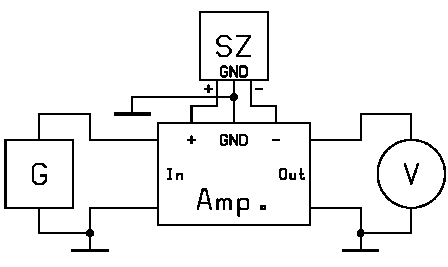
\includegraphics[scale=0.7]{schema.png}
\caption{Reálné schéma zapojení}
\end{figure}

\section{Naměřené a vypočítané hodnoty}
\begin{table}[H]
\caption{Hloubky, Výšky - střed}
\begin{tabular}{|c|c|c|c|c|c|c|c|c|c|c|}
\hline 
$f\,[Hz]$ & 16 & 50 & 100 & 500 & 800 & 1k & 2k & 4k & 8k & 16k \\ 
\hline 
$\Delta a_u\,[dB]$ & -0,4 & 0 & -0,15 & -0,1 & -0,01 & 0 & 0 & -0,1 & -0,2 & -0,25 \\ 
\hline 
\end{tabular} 
\end{table}

\begin{table}[H]
\caption{Hloubky, Výšky - minimum}
\begin{tabular}{|c|c|c|c|c|c|c|c|c|c|c|}
\hline 
$f\,[Hz]$ & 16 & 50 & 100 & 400 & 800 & 1k & 2k & 4k & 8k & 16k \\ 
\hline 
$\Delta a_u\,[dB]$ & -22 & -18 & -11 & -2,1 & -0,11 & -0,9 & -1,8 & -4,1 & -8,8 & -15 \\ 
\hline 
\end{tabular} 
\end{table}

\begin{table}[H]
\caption{Hloubky, Výšky - maximum}
\begin{tabular}{|c|c|c|c|c|c|c|c|c|c|c|}
\hline 
$f\,[Hz]$ & 16 & 50 & 100 & 400 & 800 & 1k & 2k & 4k & 8k & 16k \\ 
\hline 
$\Delta a_u\,[dB]$ & 19 & 16 & 11 & 2 & 1 & 1 & 1,9 & 4,5 & 9 & 14 \\ 
\hline 
\end{tabular} 
\end{table}

\section{Grafy}
\begin{figure}[H]
\centering
	\begin{tikzpicture}
		%\begin{axis}[
			
		\begin{semilogxaxis}[
			width=1\textwidth,
	     	height=0.9\textwidth,
			xlabel={$f\,[Hz]$},
			ylabel={$\Delta a_u\,[dB]$}
		]
			
		\addplot coordinates {
			(16,-0.4)
			(50,0)
			(100,-0.15)
			(500,-0.1)
			(800,-0.01)
			(1000,0)
			(2000,0)
			(4000,-0.1)
			(8000,-0.2)
			(16000,-0.25)
		};
		\addlegendentry{střed}
		
		\addplot coordinates {
			(16,-22)
			(50,-18)
			(100,-11)
			(400,-2.1)
			(800,-0.11)
			(1000,-0.9)
			(2000,-1.8)
			(4000,-4.1)
			(8000,-8.8)
			(16000,-15)
		};
		\addlegendentry{minimum}
		
		\addplot coordinates {
			(16,19)
			(50,16)
			(100,11)
			(400,2)
			(800,1)
			(1000,1)
			(2000,1.9)
			(4000,4.5)
			(8000,9)
			(16000,14)
		};
		\addlegendentry{maximum}
		
		\end{semilogxaxis}
	\end{tikzpicture}
	\caption{Přenosové kmitočtové charakterisitky pro mezní polohy korekce}
\end{figure}

Šířku pásma $B$ určíme ze vztahu $B = f_H - f_L$, kde $f_H$ je horní a $f_L$ dolní frekvence odpovídající poklesu zisku o $3\,dB$ od referenční úrovně. Pro obě mezní polohy korekce jsou odpovídající frekvence přibližně stejné a to $f_H = 3000\,Hz$ a $f_L = 300\,Hz$, takže šířka pásma $B = f_H - f_L = 3000 - 300 = 2700\,Hz$.

Na obrázcích níže lze vidět účinky předzesilovače na obdélníkový signál při použití například RC pásmové propusti. Vždy dochází k jinému zkreslení v závislosti na tom, jestli filtrem potlačujeme vysoké, nebo nízké frekvence.

\begin{figure}[H]
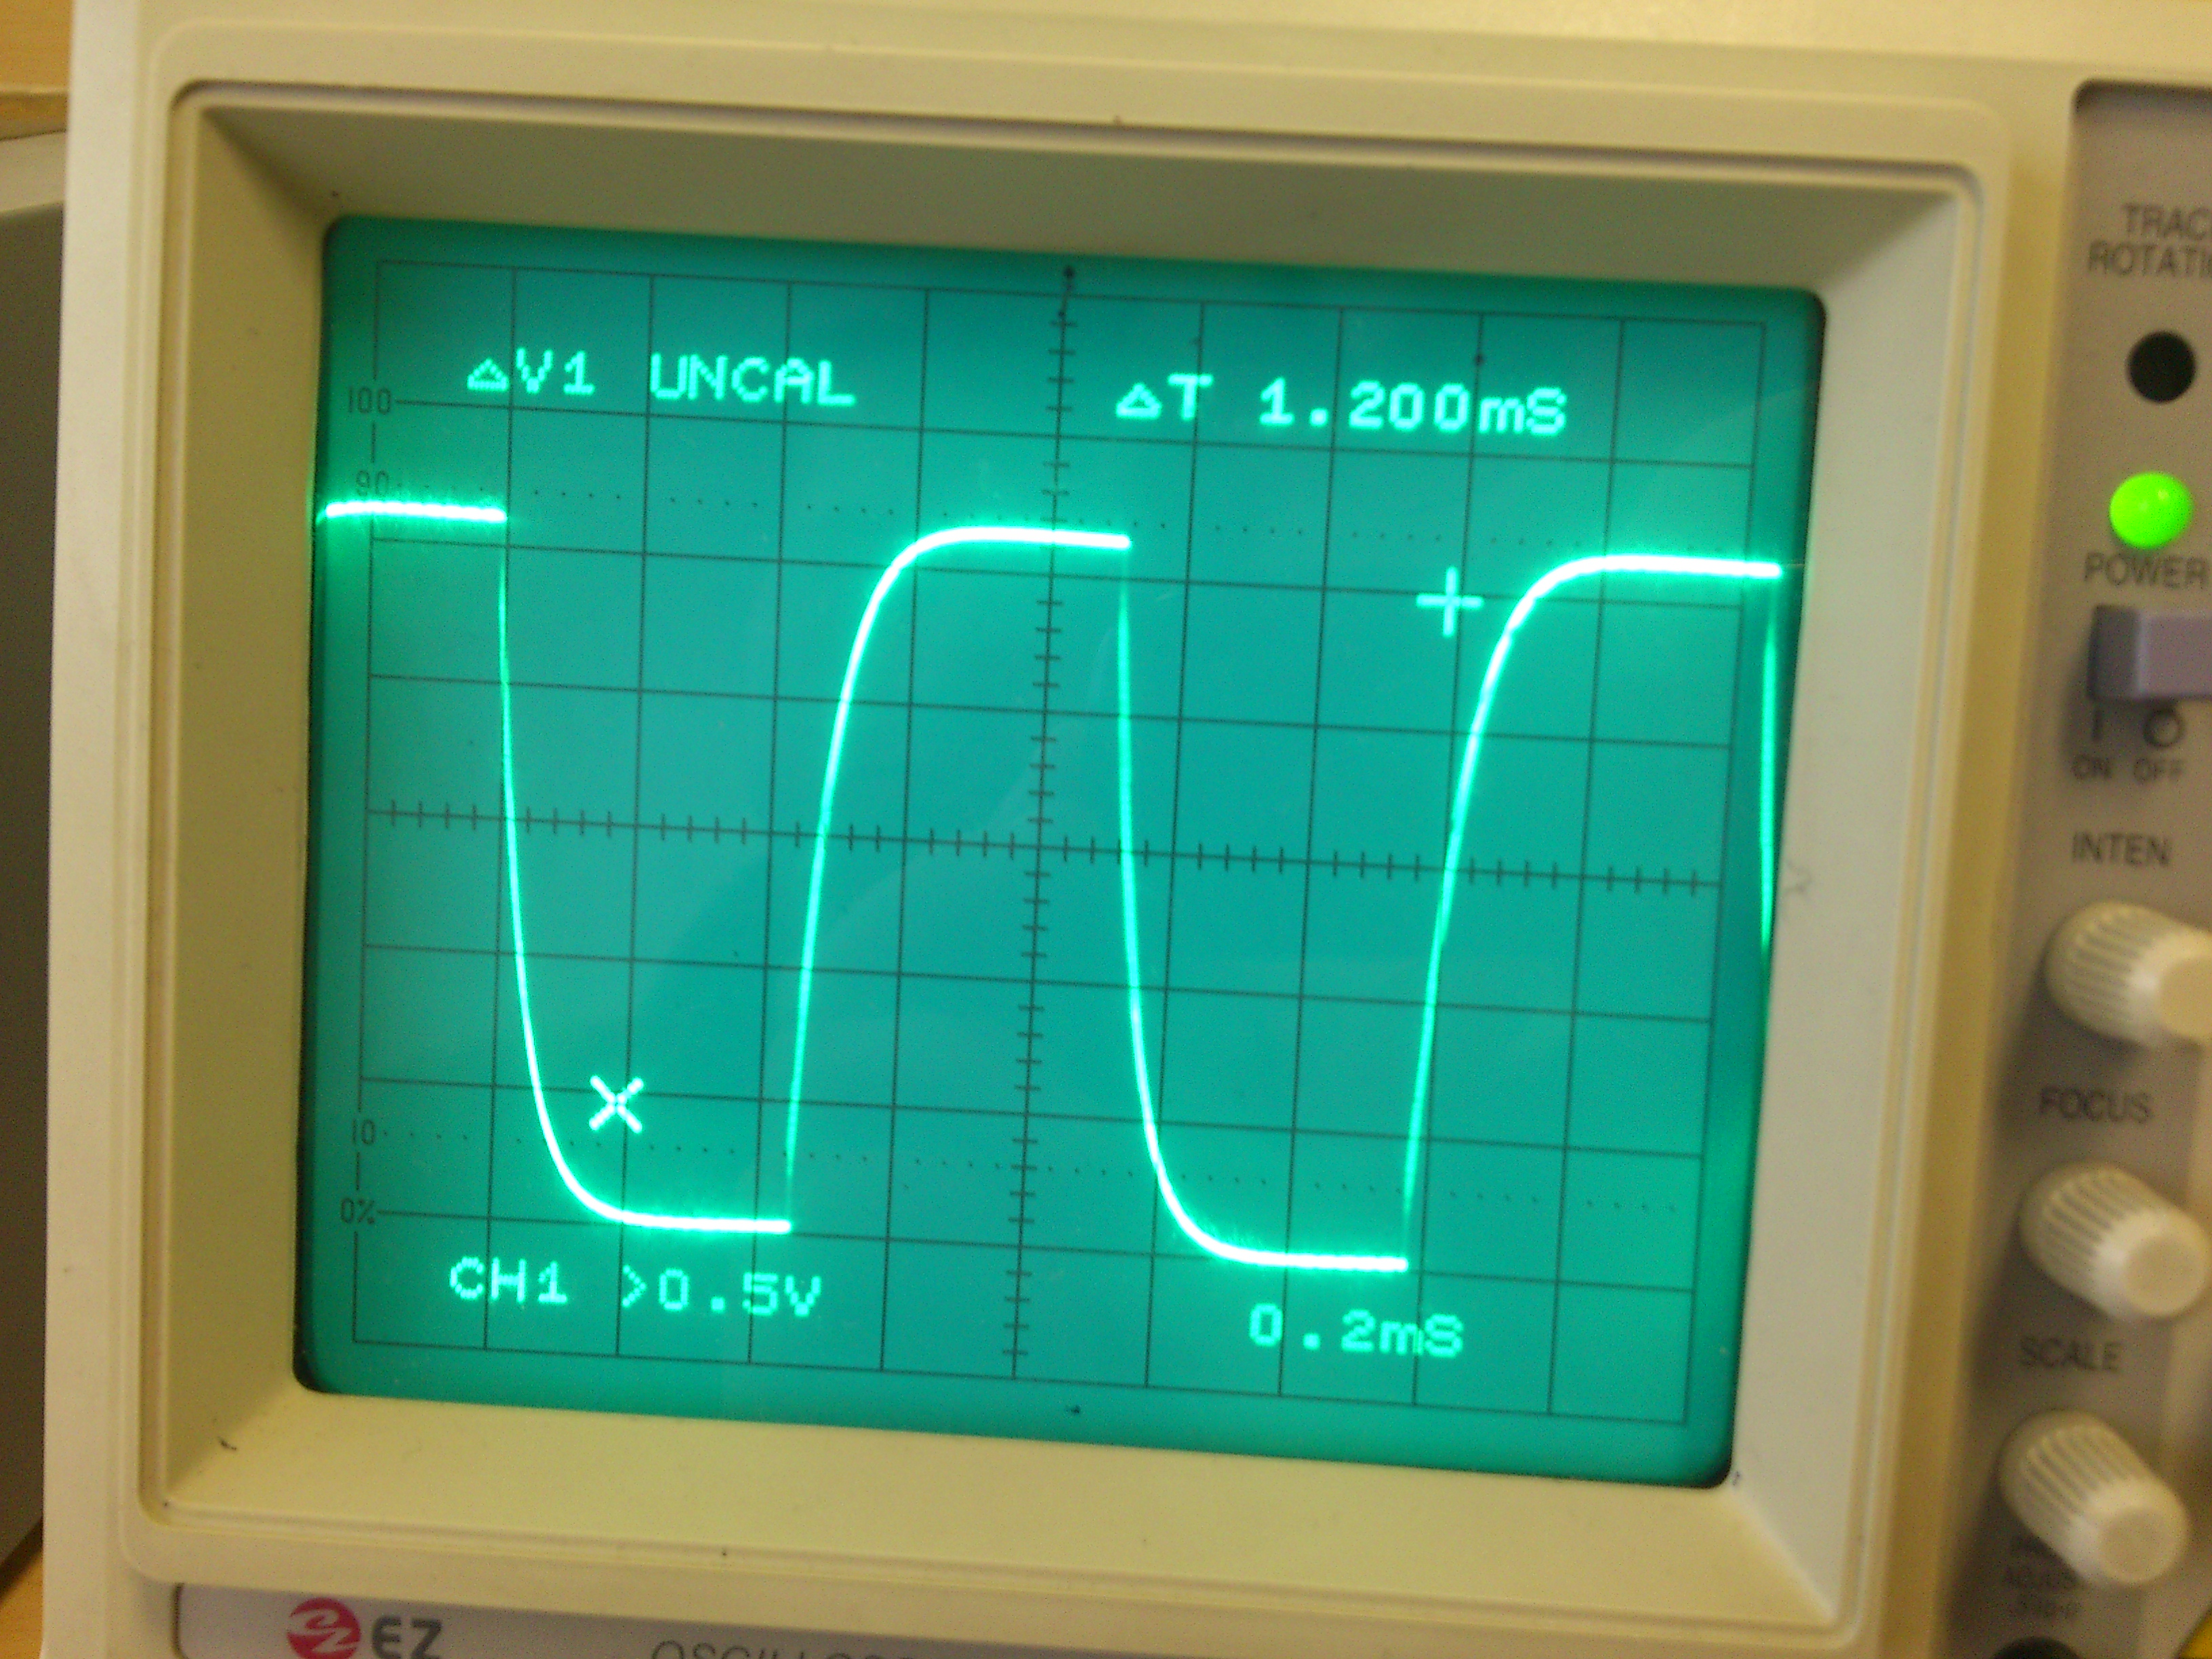
\includegraphics[scale=0.065]{IMG_20131119_133630.jpg}
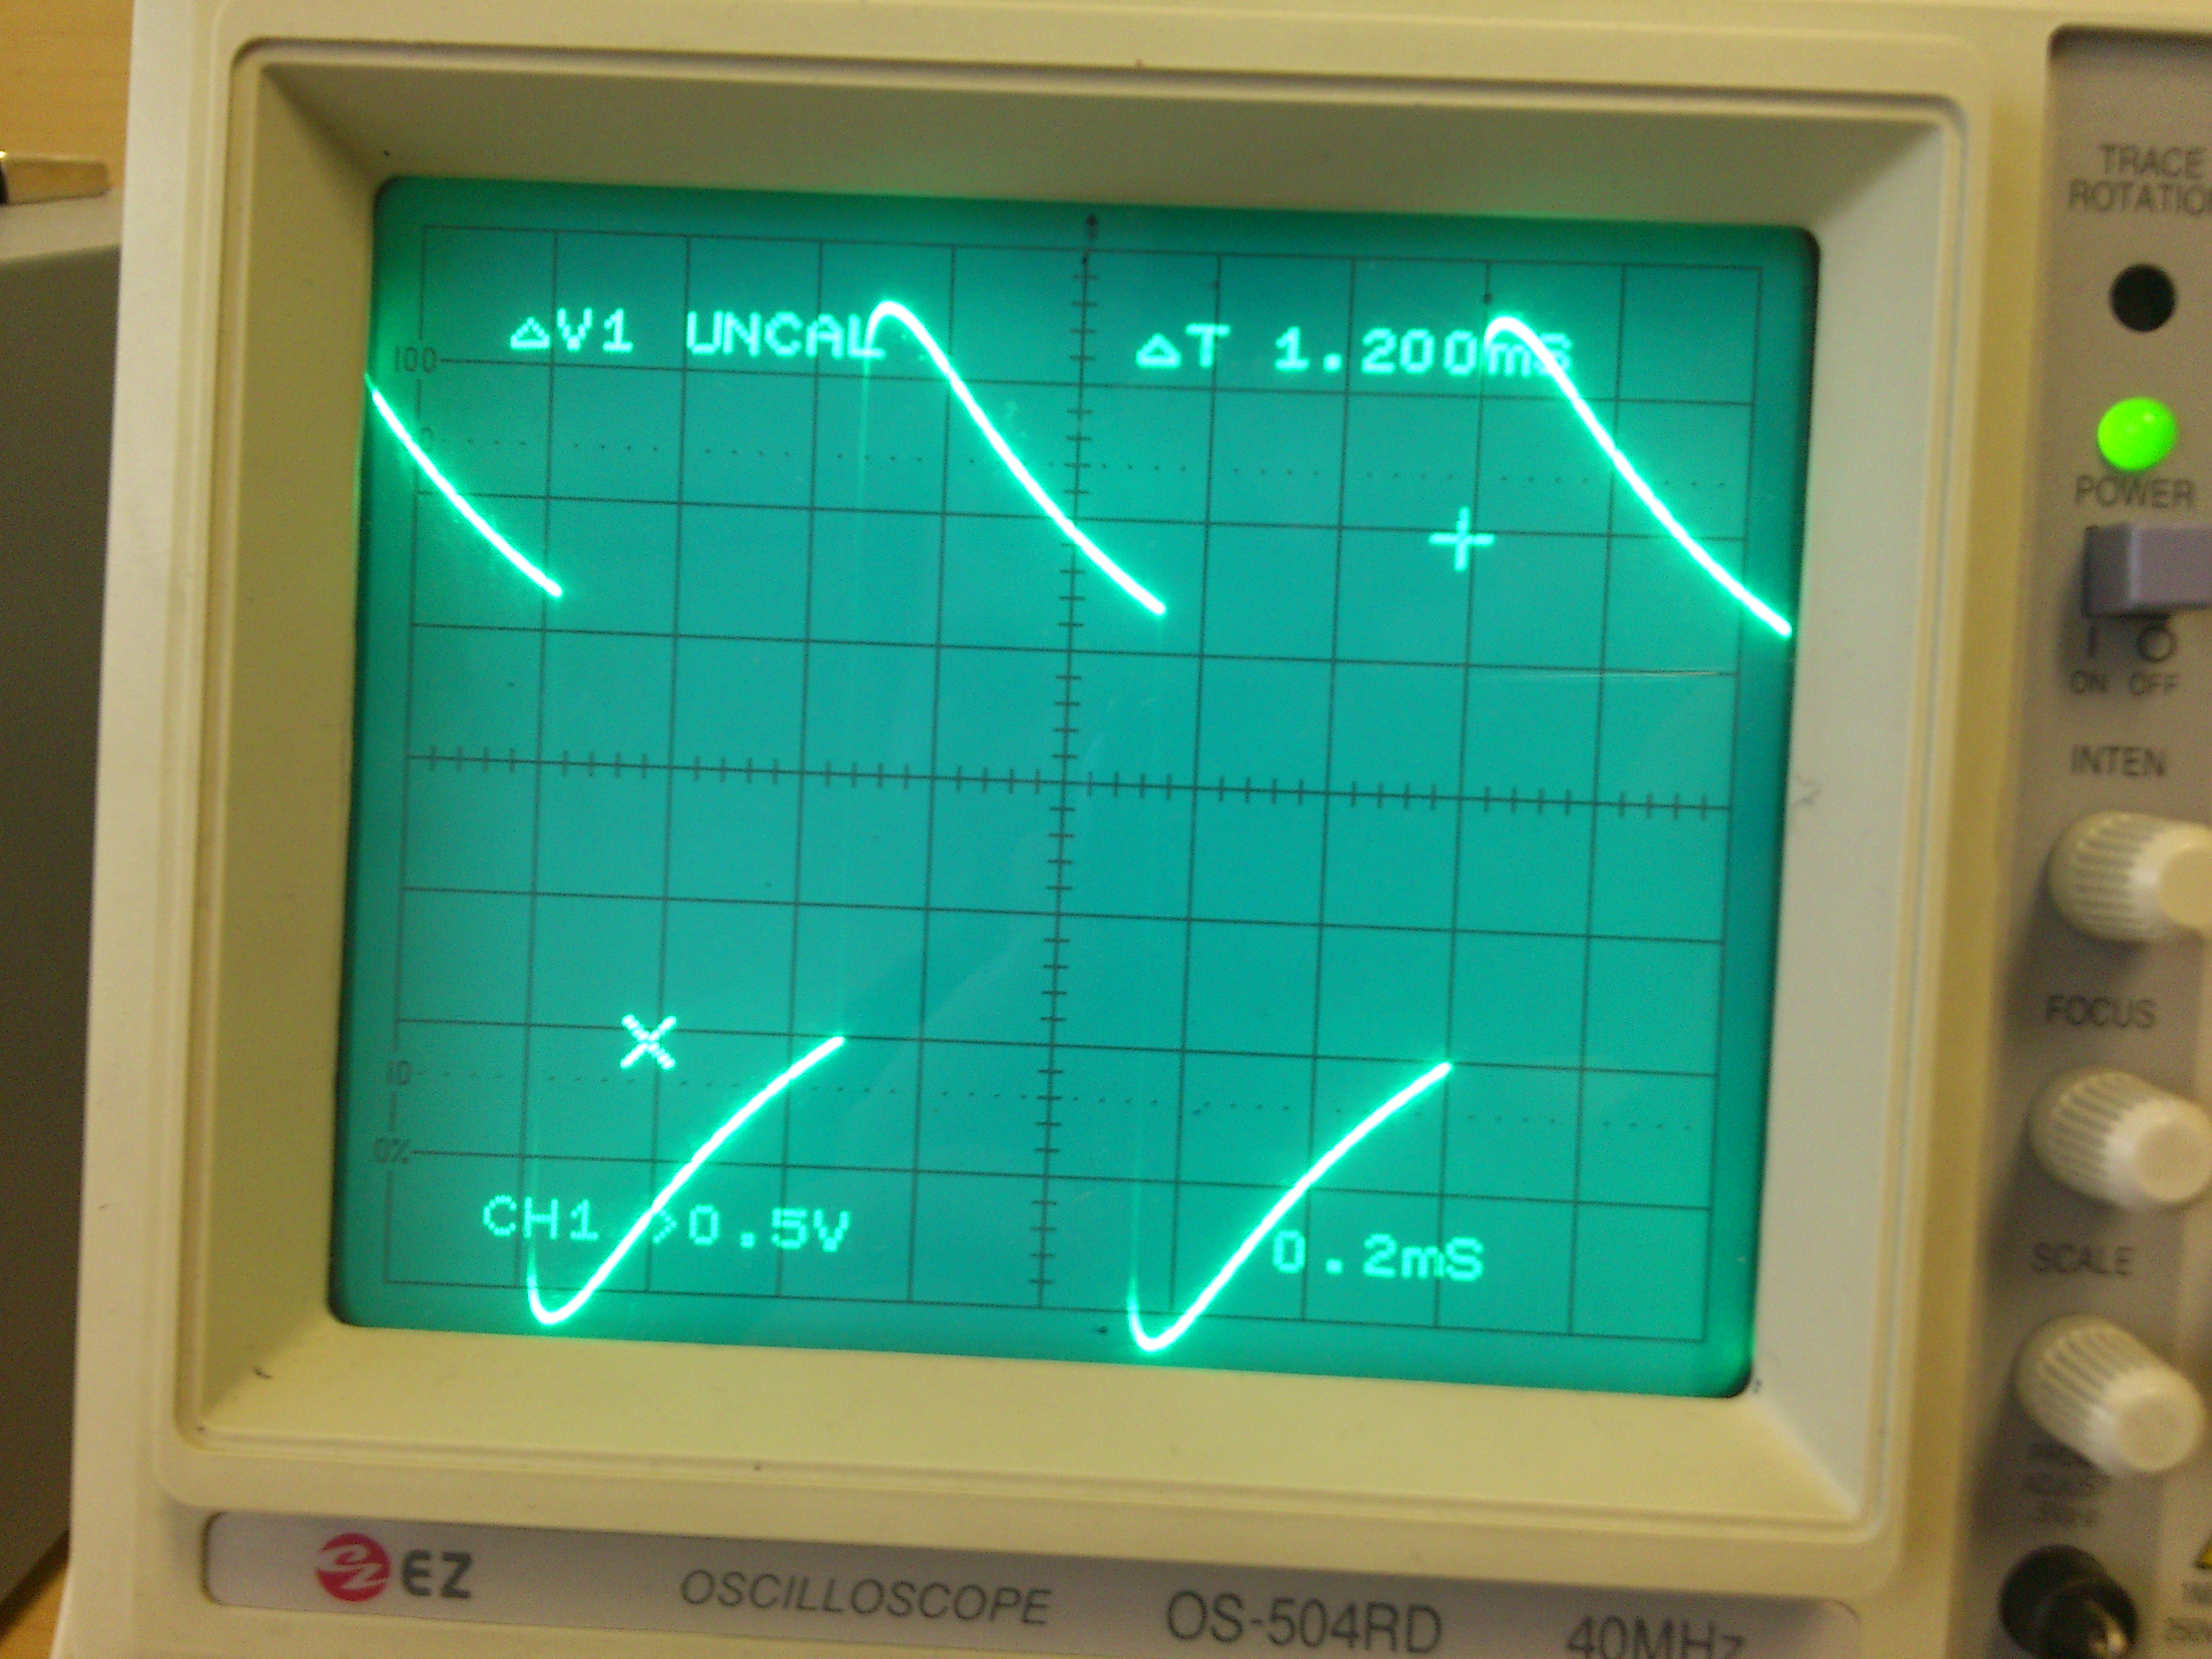
\includegraphics[scale=0.065]{IMG_20131119_133652.jpg}
\caption{Potlačení vysokých, resp. nízkých frekvencí}
\end{figure}

Obdobně je tomu i na následujících obrázcích, zde však dochází k zesilování vysokých, nebo nízkých frekvencí. Jak je vidět, tak to odpovídá přesnému opaku předchozího případu. Tam kde původně byla část kmitu potlačena, tam je nyní zesílena a naopak.

\begin{figure}[H]
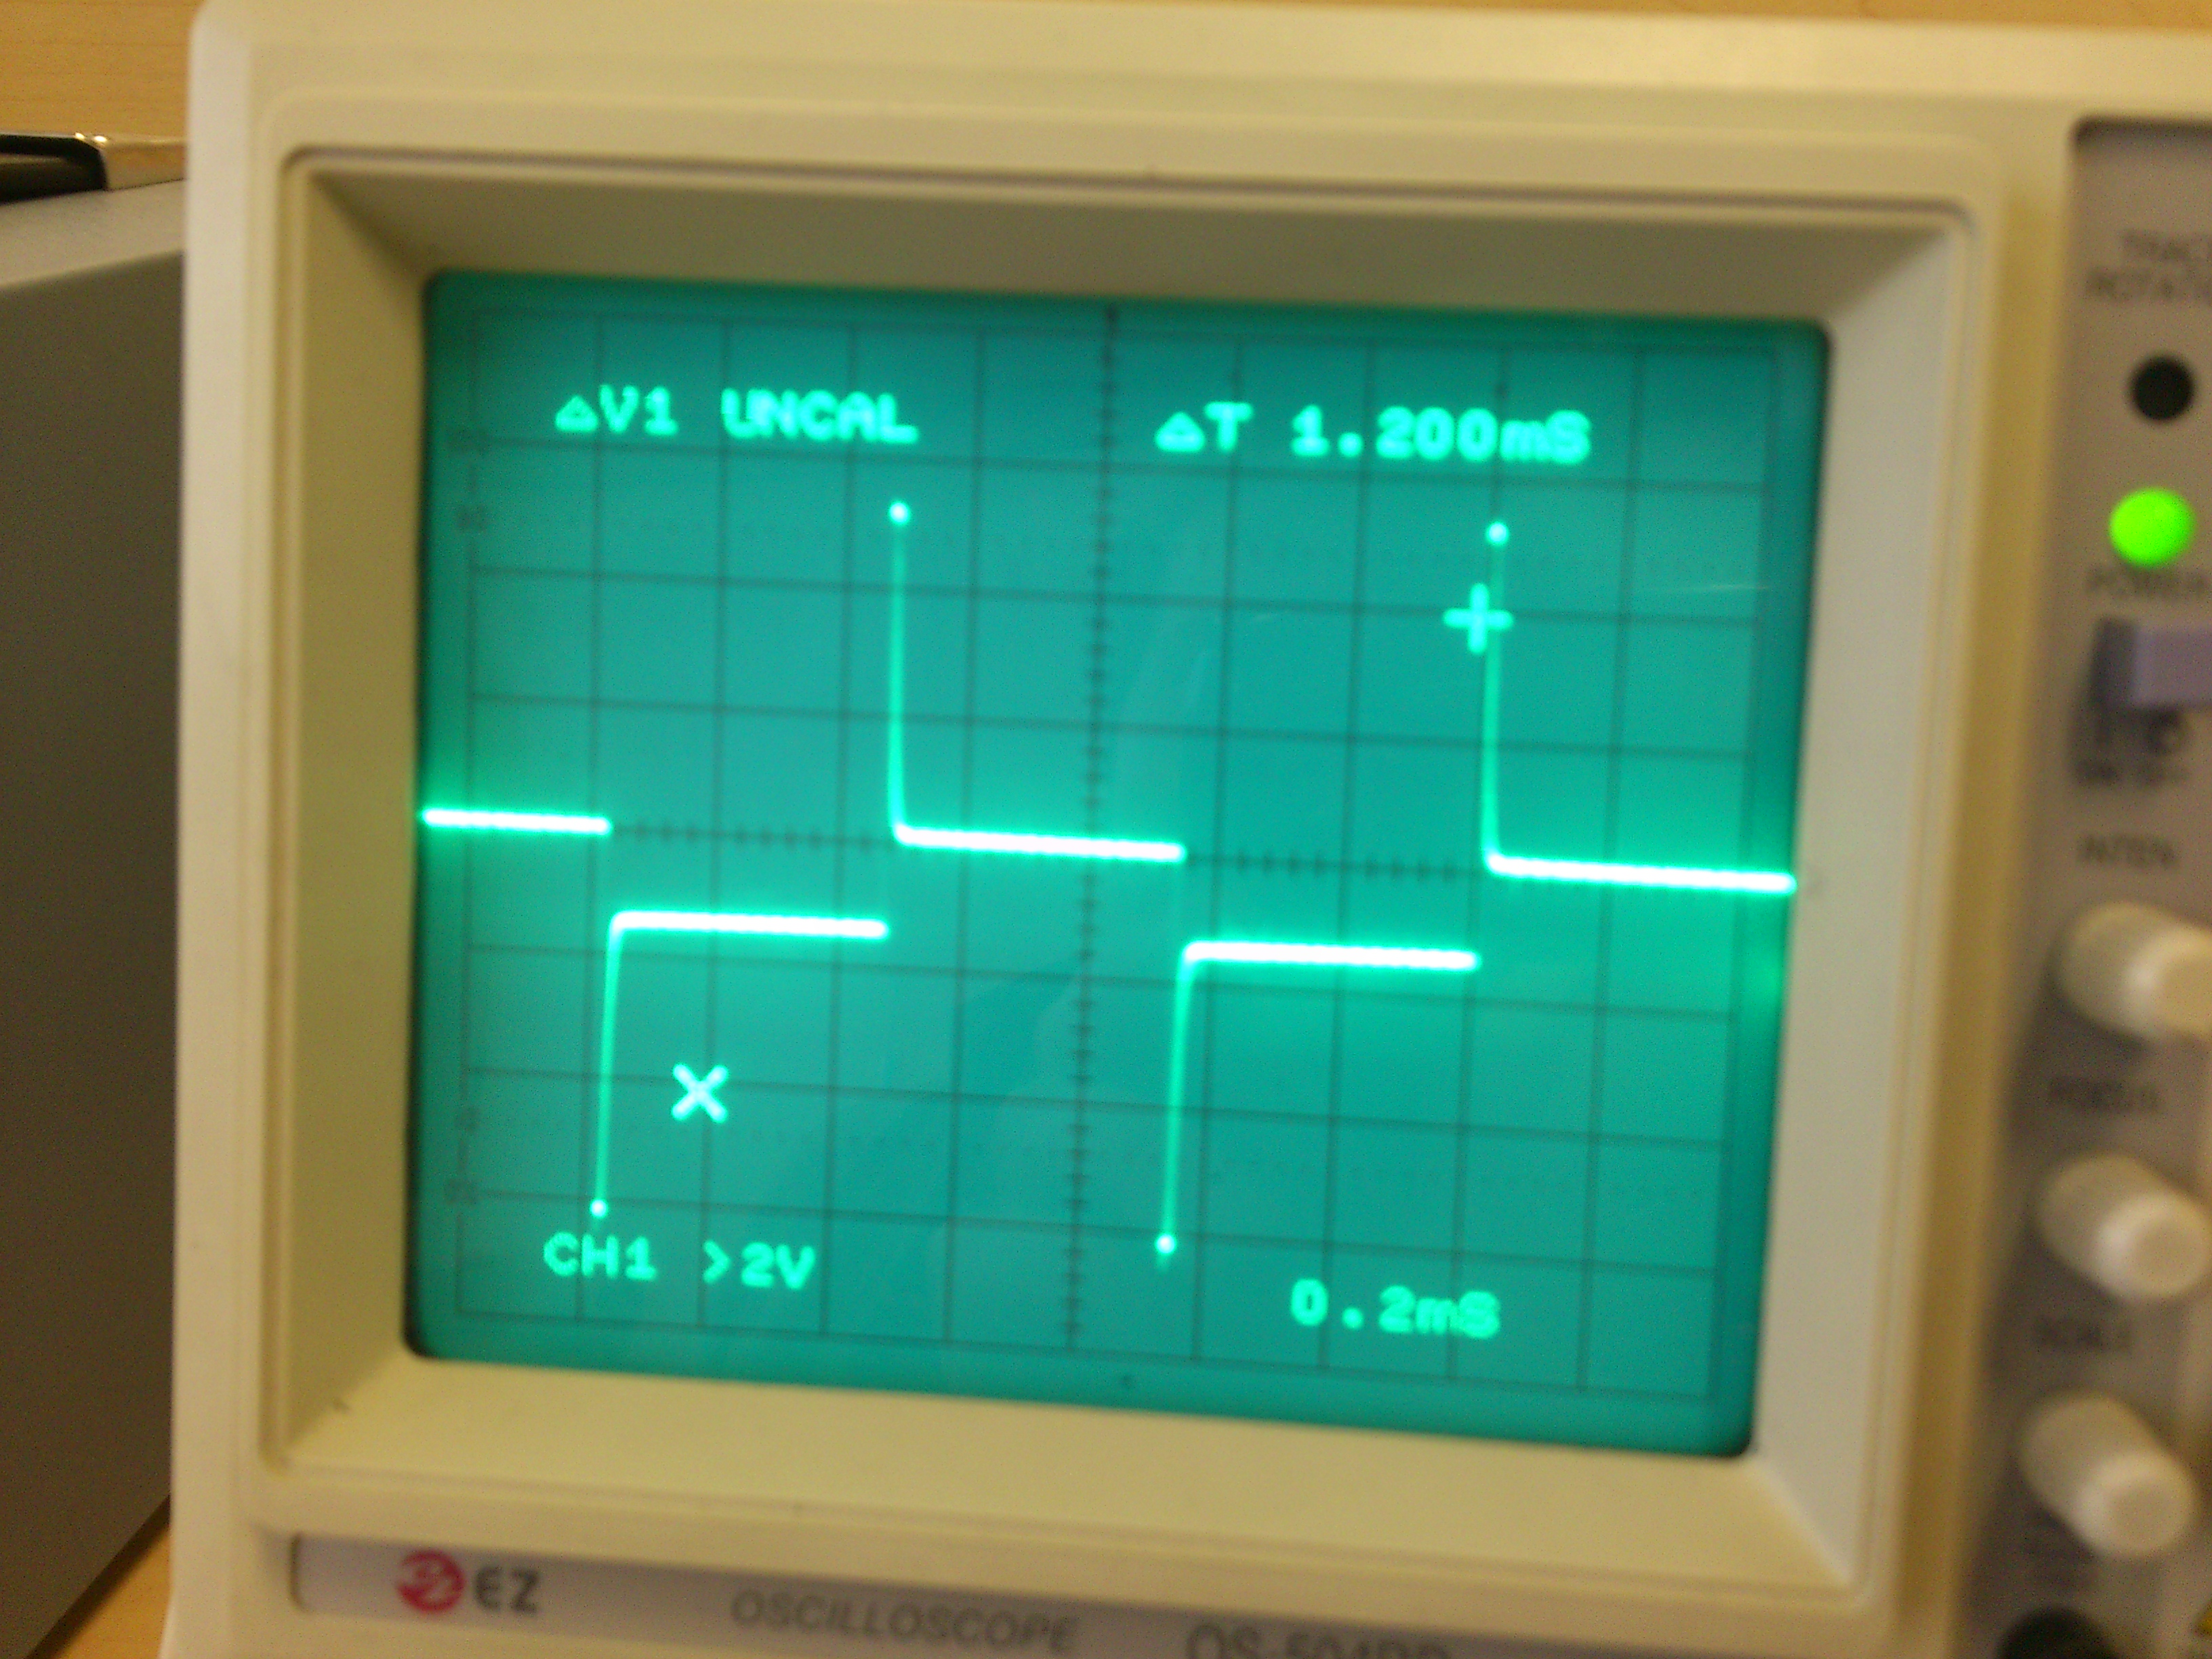
\includegraphics[scale=0.065]{IMG_20131119_133755.jpg}
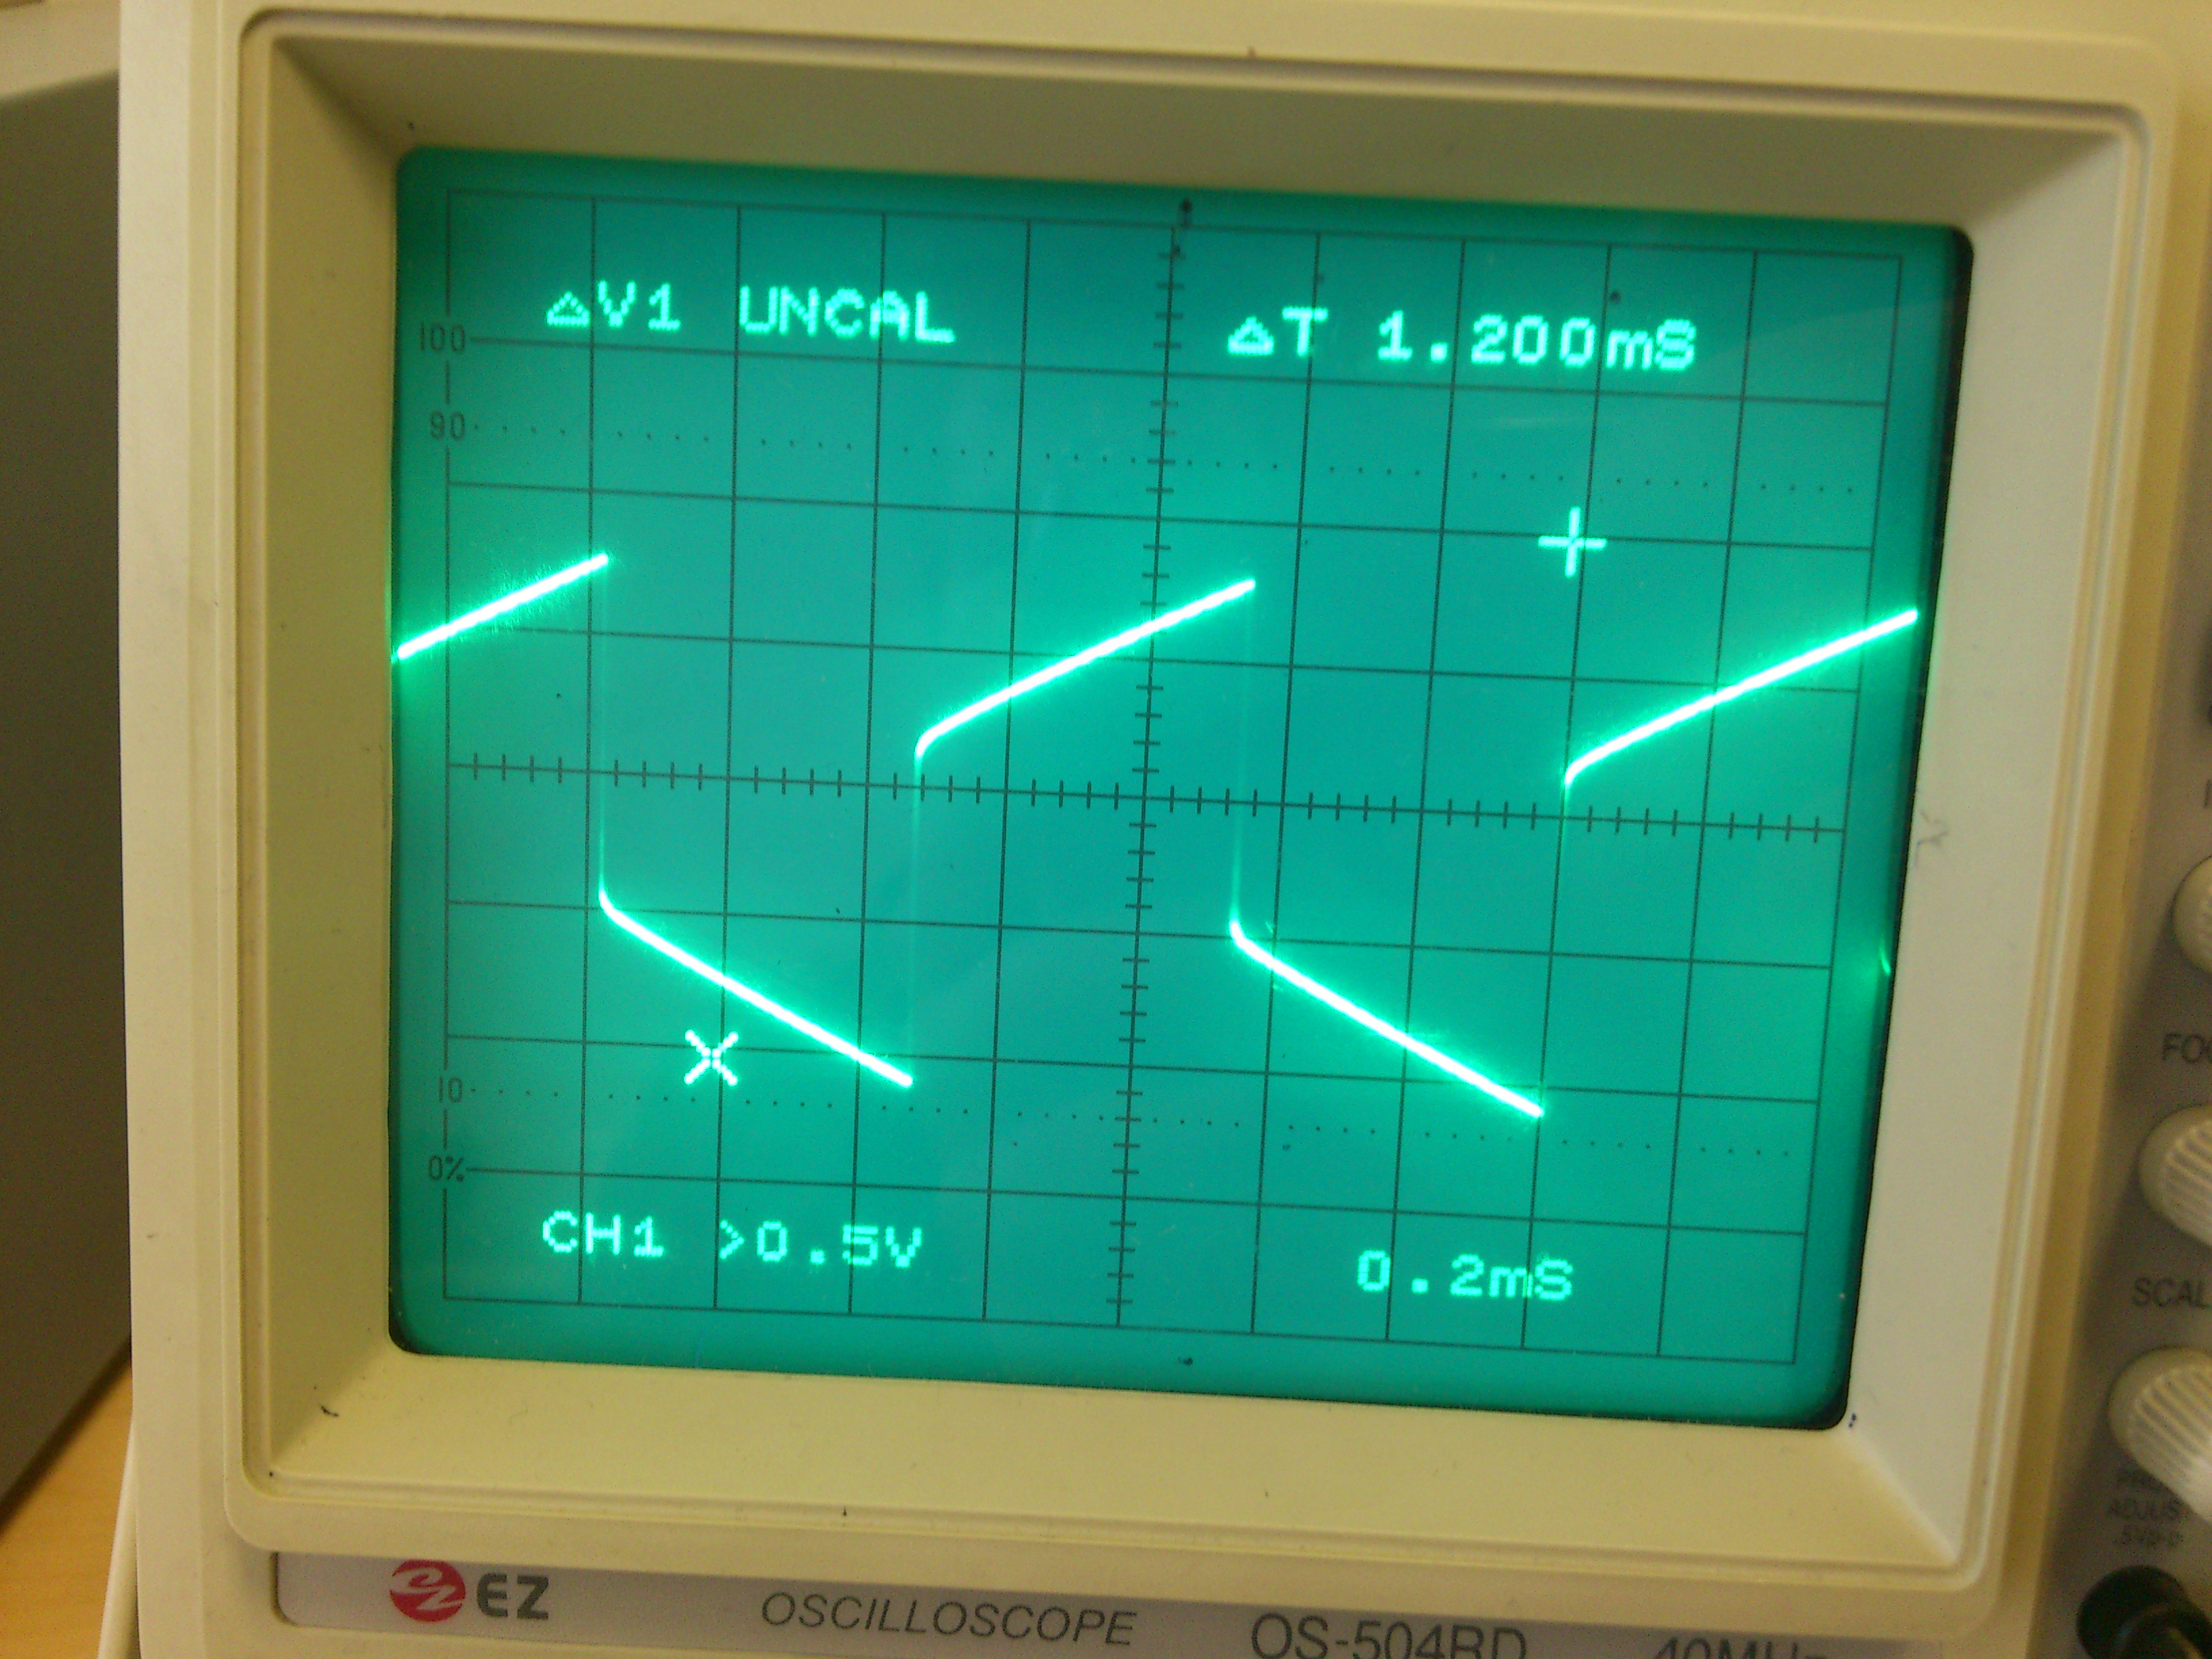
\includegraphics[scale=0.065]{IMG_20131119_133807.jpg}
\caption{Zesílení vysokých, resp. nízkých frekvencí}
\end{figure}

Sloučením zesílení jak vysokých, tak nízkých frekvencí získáme následující obrázky. Stejně je tomu pro potlačení frekvencí. Výsledné průběhy odpovídají sloučením předchozích dvou průběhů vždy příslušejících k danému zesílení, resp. potlačení.

\begin{figure}[H]
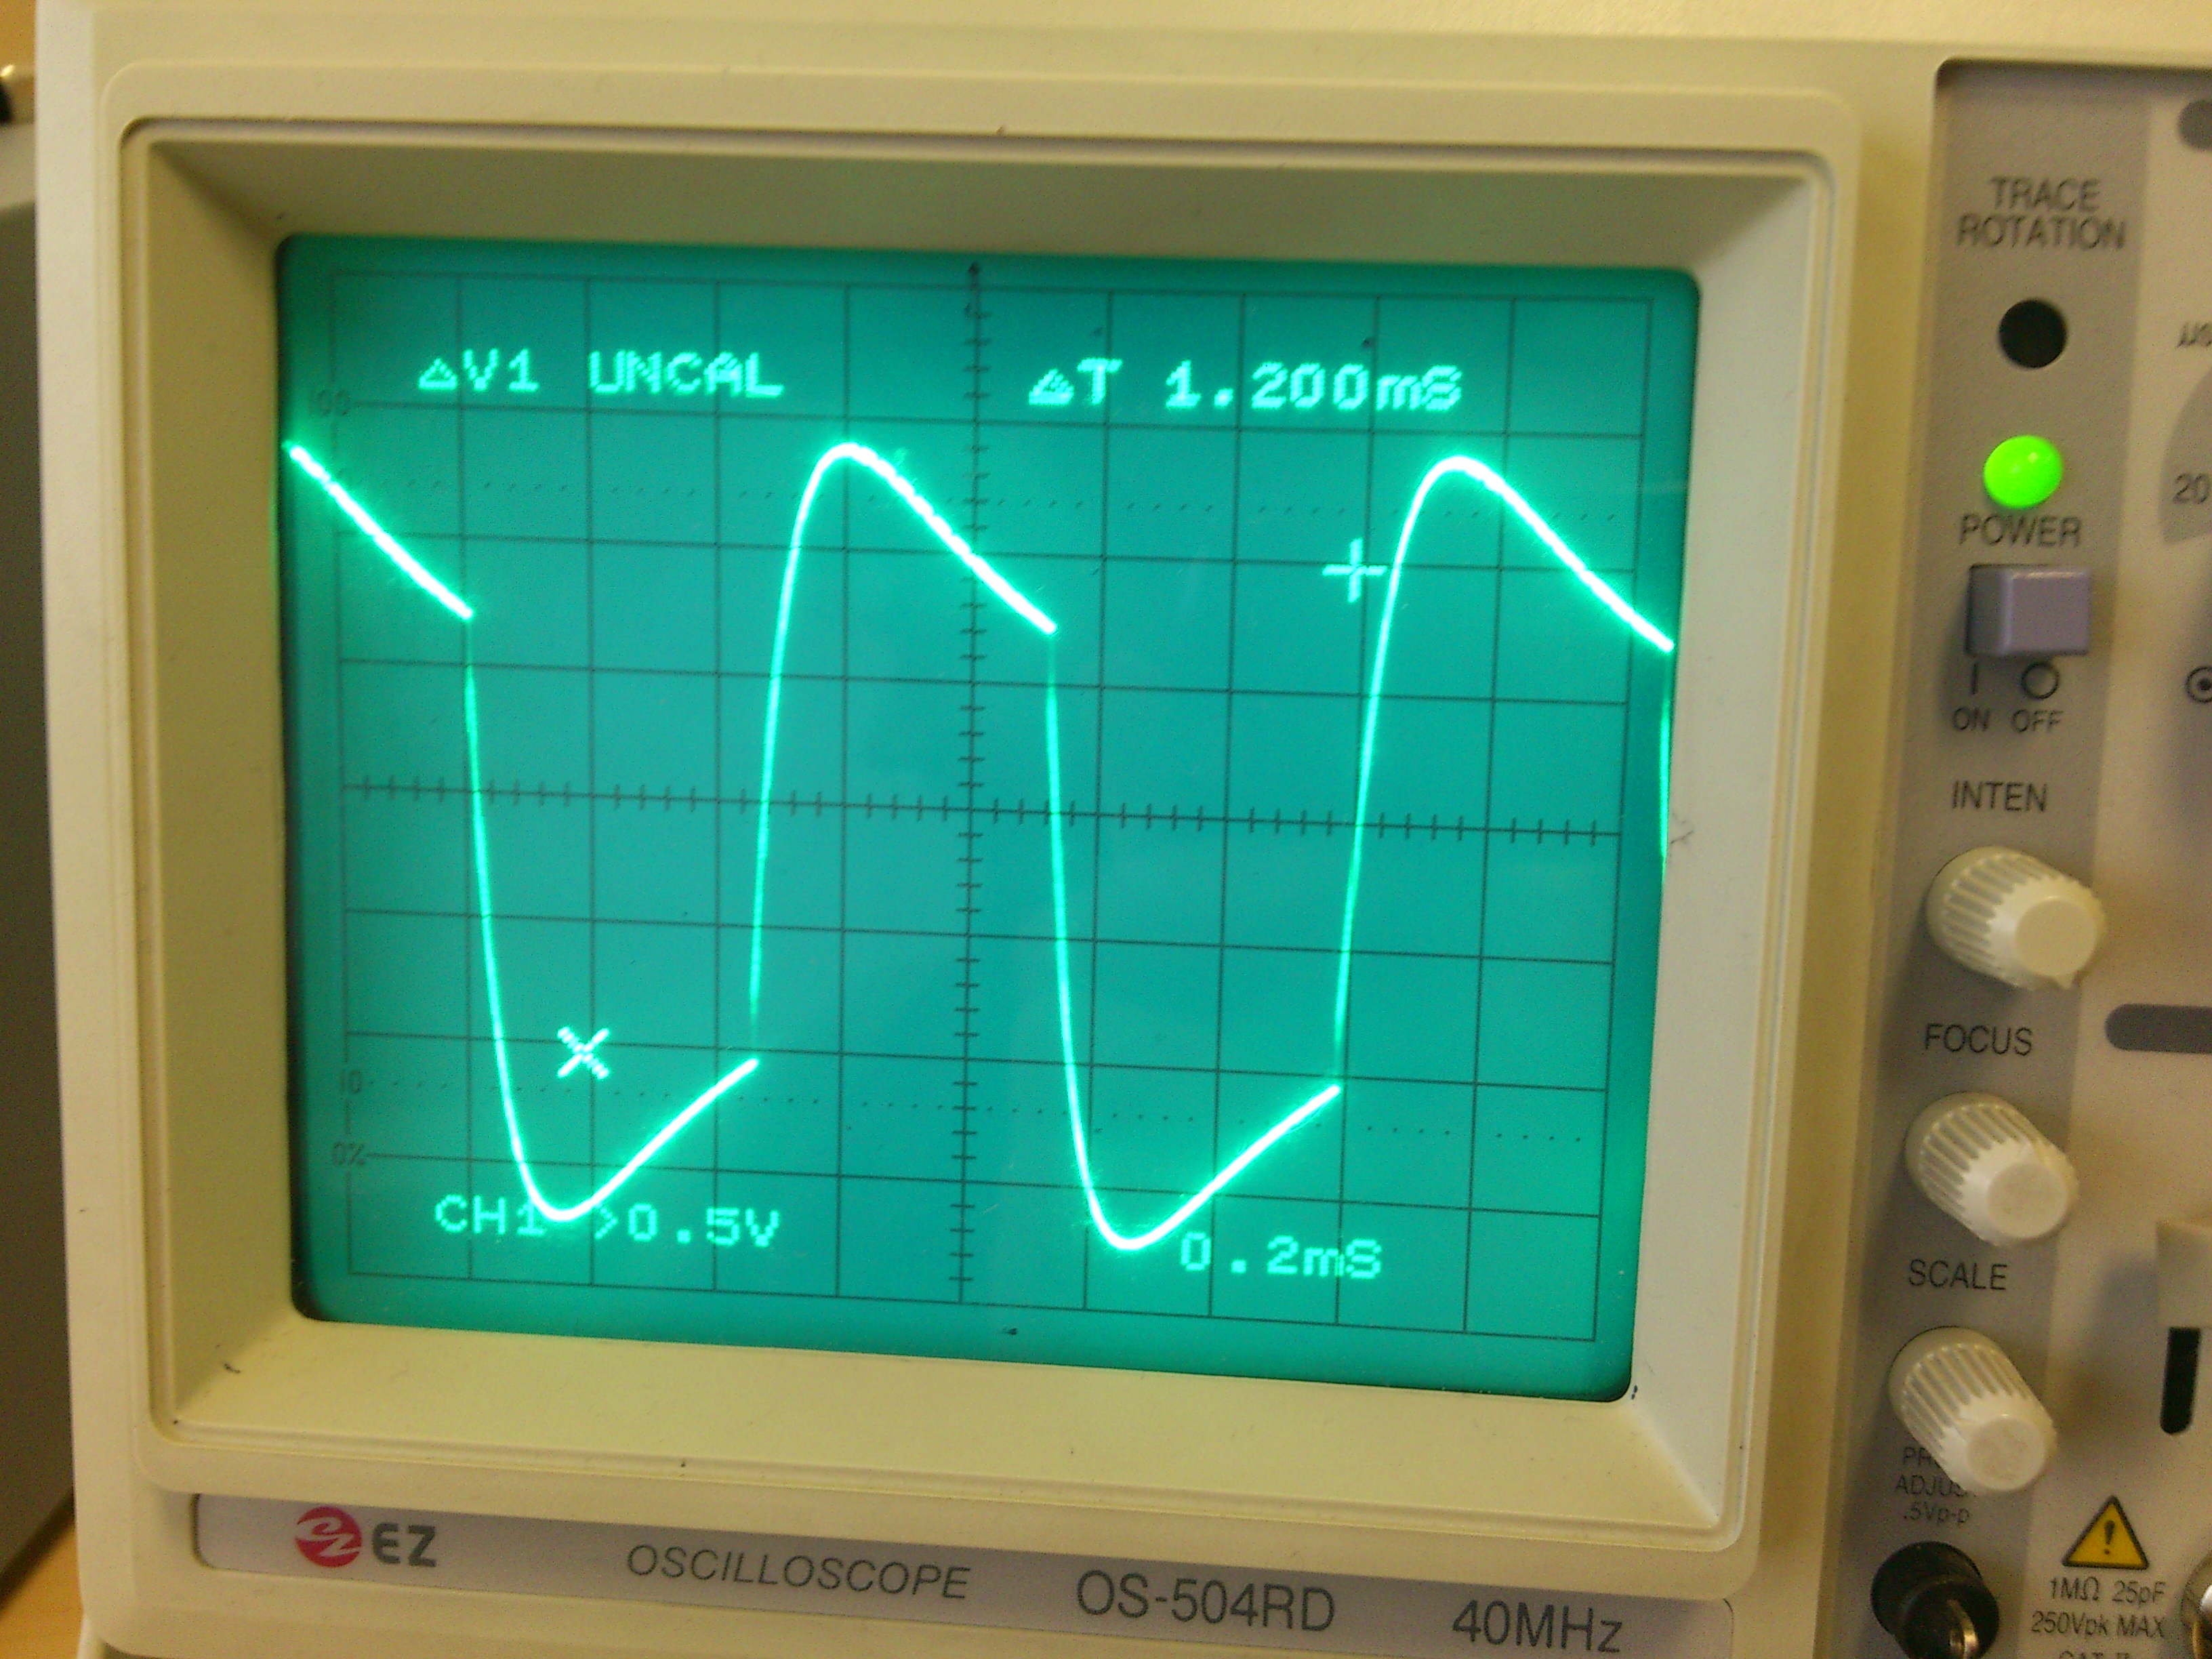
\includegraphics[scale=0.065]{IMG_20131119_133721.jpg}
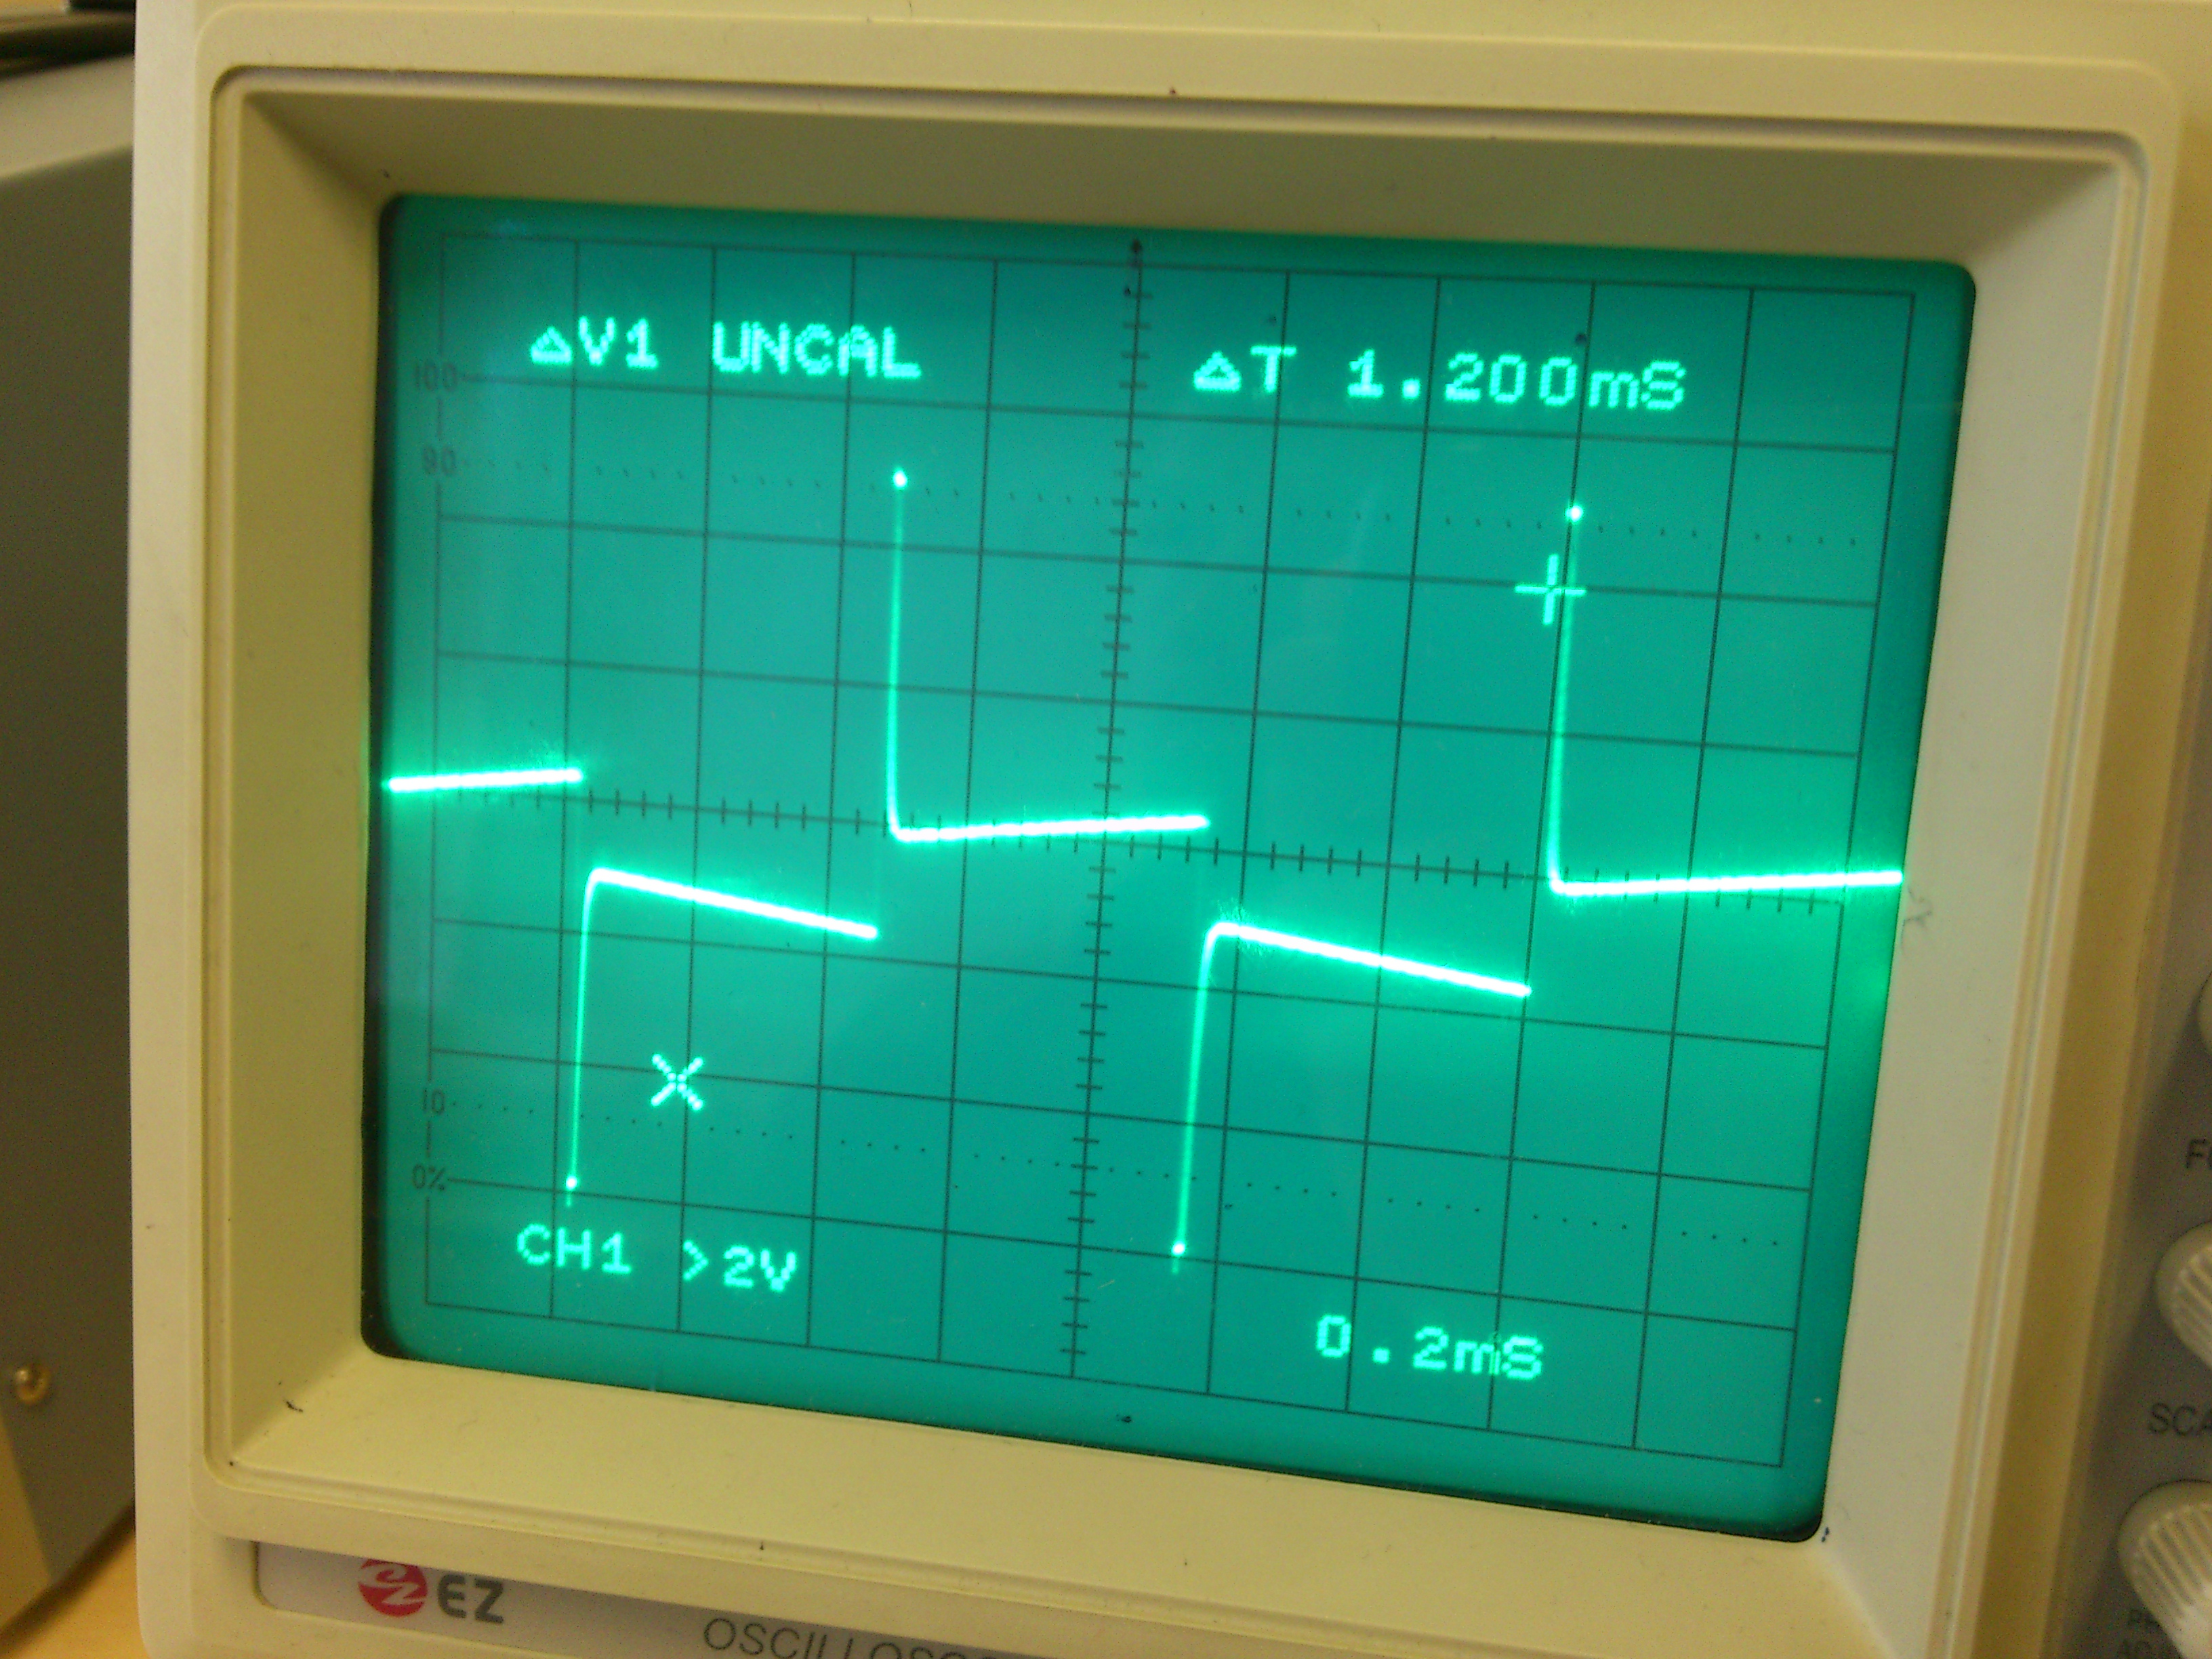
\includegraphics[scale=0.065]{IMG_20131119_133835.jpg}
\caption{Potlačení, resp. zesílení vysokých a nízkých frekvencí}
\end{figure}

\section{Závěr}
Šířka pásma zesilovače pro obě nastavení korekcí je přibližně $2700\,Hz$. Vzrůst resp. pokles zisku vůči zisku na referenčním kmitočtu což je v našem případě $1\,kHz$ je vidět z grafu. Při referenčním kmitočku k žádnému zvrůstu ani poklesu nedochází, oproti tomu v mezních kmitočtech měření k těmto vzrůstům, resp. poklesům dochází a to souměrně podle referenční hodnoty $0\,dB$.

\section{Přístroje}
\begin{itemize}
\item Generátor funkcí FG-7002C, evid. 109716
\item NF předzesilovač, evid. 117246
\item dB meter TVT-321, evid. 109143
\item Stabilizovaný napájecí zdroj
\end{itemize}

\end{document}
